\documentclass{beamer}

\begin{document}
\huge
\centering
\begin{frame}{}
\[ 2+7=9 \] \\ 
\vspace{30pt}
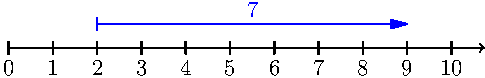
\includegraphics[scale=1.25]{/home/sindre/openmathbooks/MB/fig/plus2}
\end{frame}	

\begin{frame}{}
	\[ 6-4=2 \] \\ 
	\vspace{30pt}
	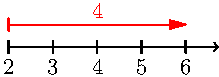
\includegraphics[scale=1.25]{/home/sindre/openmathbooks/MB/fig/mint}
\end{frame}	

\begin{frame}{}
\large
5 har lengde 5 og retning mot \textsl{høgre}.\\[12pt]
$ -5 $ har lengde 5 og retning mot \textsl{venstre}. \\[12pt]
	\vspace{30pt}
	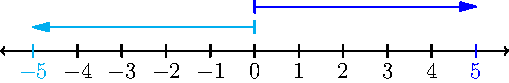
\includegraphics[scale=1.25]{/home/sindre/openmathbooks/MB/fig/neg3}
\end{frame}	

\begin{frame}{}
	\[ 7+(-4)=3 \] \\ 
	\vspace{30pt}
	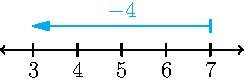
\includegraphics[scale=1.25]{/home/sindre/openmathbooks/MB/fig/neg6}
\end{frame}	

\begin{frame}{}
	\[ 2-(-6)=8 \] \\ 
	\vspace{30pt}
	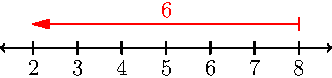
\includegraphics[scale=1.25]{/home/sindre/openmathbooks/MB/fig/neg7}
\end{frame}	

\end{document}